\FloatBarrier
\subsection{Question 1}
First, we implement the open-loop system. To close the loop, we apply a minimum variance controller using \autoref{code:sstr11}. As shown in \autoref{fig:sstr11}, the system remains stable and, when actuated, returns to its equilibrium point at $0$. As shown in \autoref{fig:sstr12}, cummulative loss of the system is bounded.

\begin{code}
	\begin{matlabcode}{firstnumber = 1}
run('SSTR_0.m');

%% Diophantine equation
[F,G] = diophantine(A,C,1);

%% Open loop system
G_ol = minreal(G_discrete*tf(A,conv(B,F),Ts));

%% Closed loop system
G_cl = feedback(G_ol,1);
	\end{matlabcode}
	\captionof{listing}{Minimum variance controller}
	\label{code:sstr11}
\end{code}

\begin{figure}
	\centering
	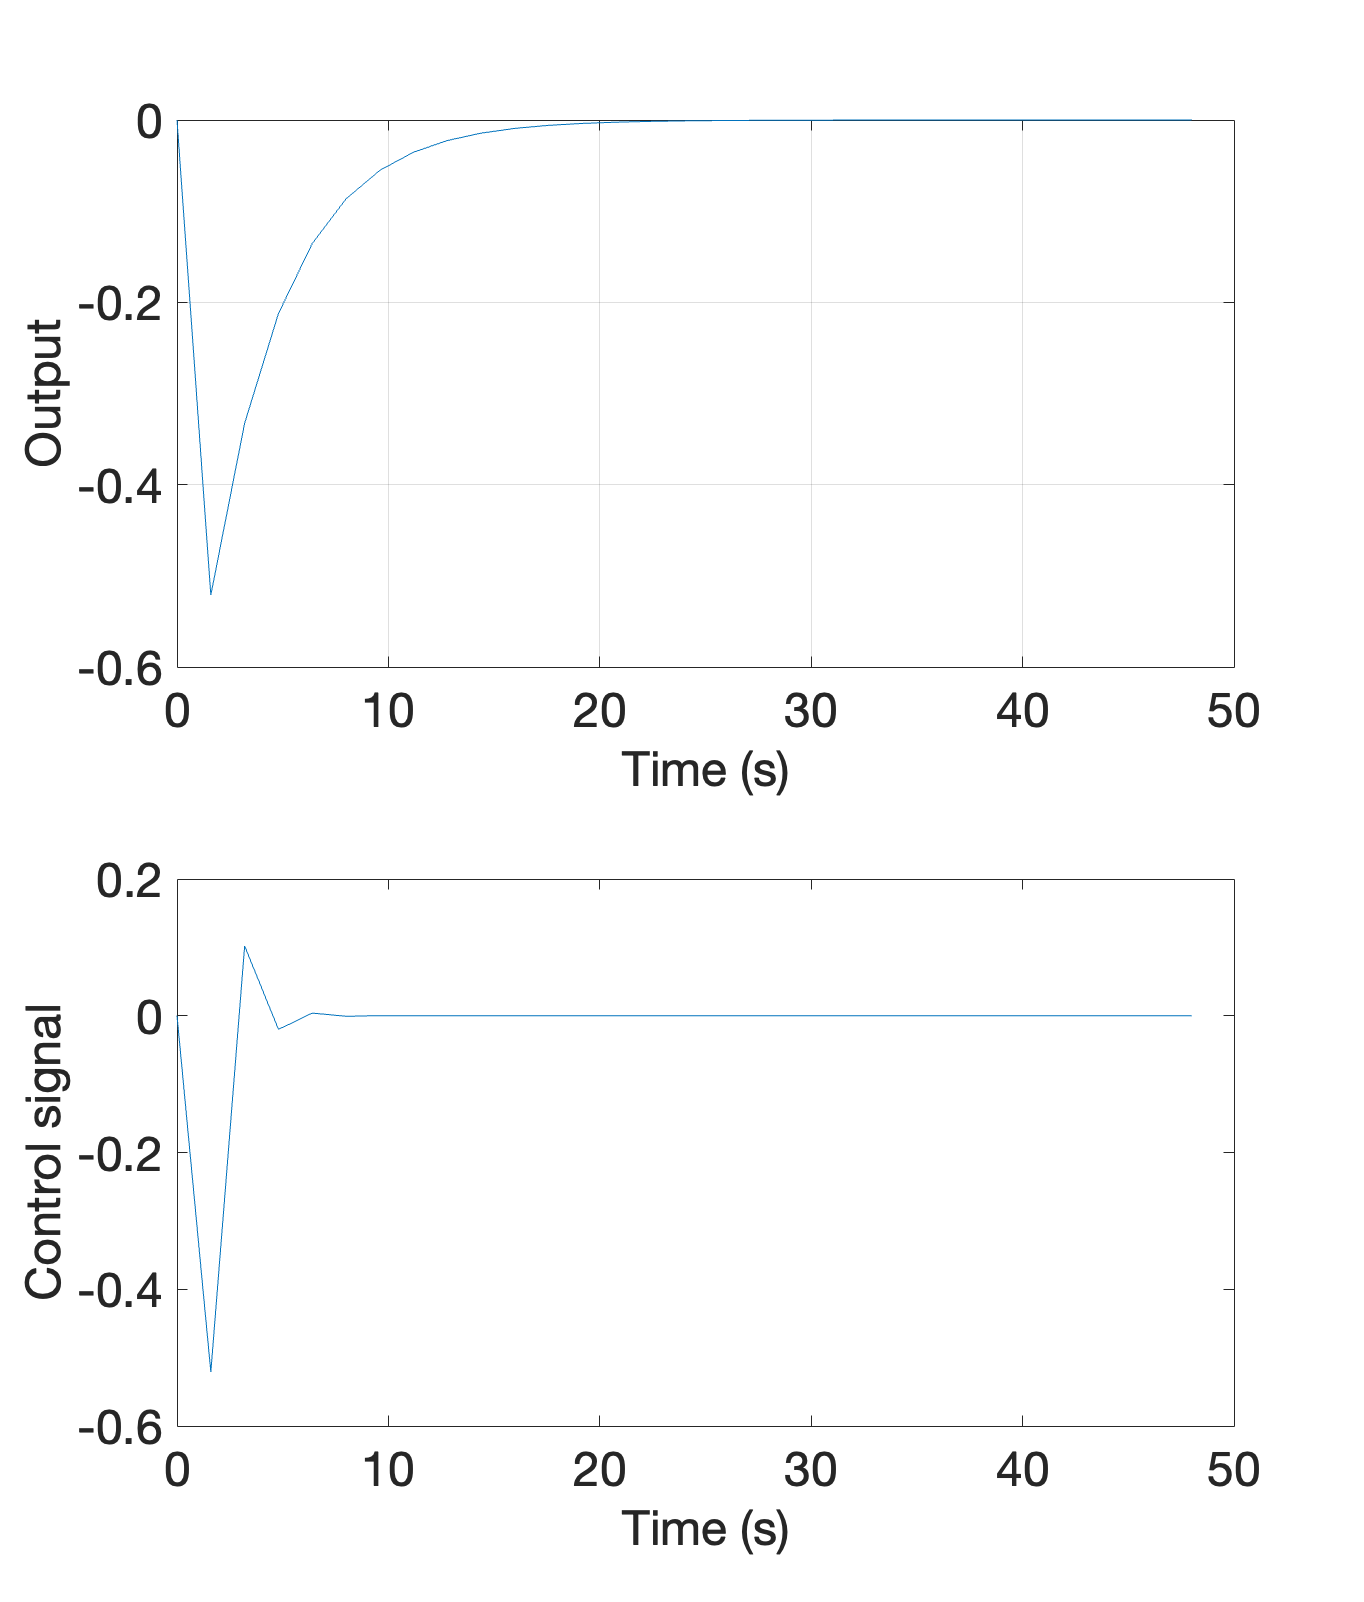
\includegraphics[width=\textwidth]{images/sstr11.png}
	\caption{Output and control of minimum variance controller}
	\label{fig:sstr11}
\end{figure}

\begin{figure}
	\centering
	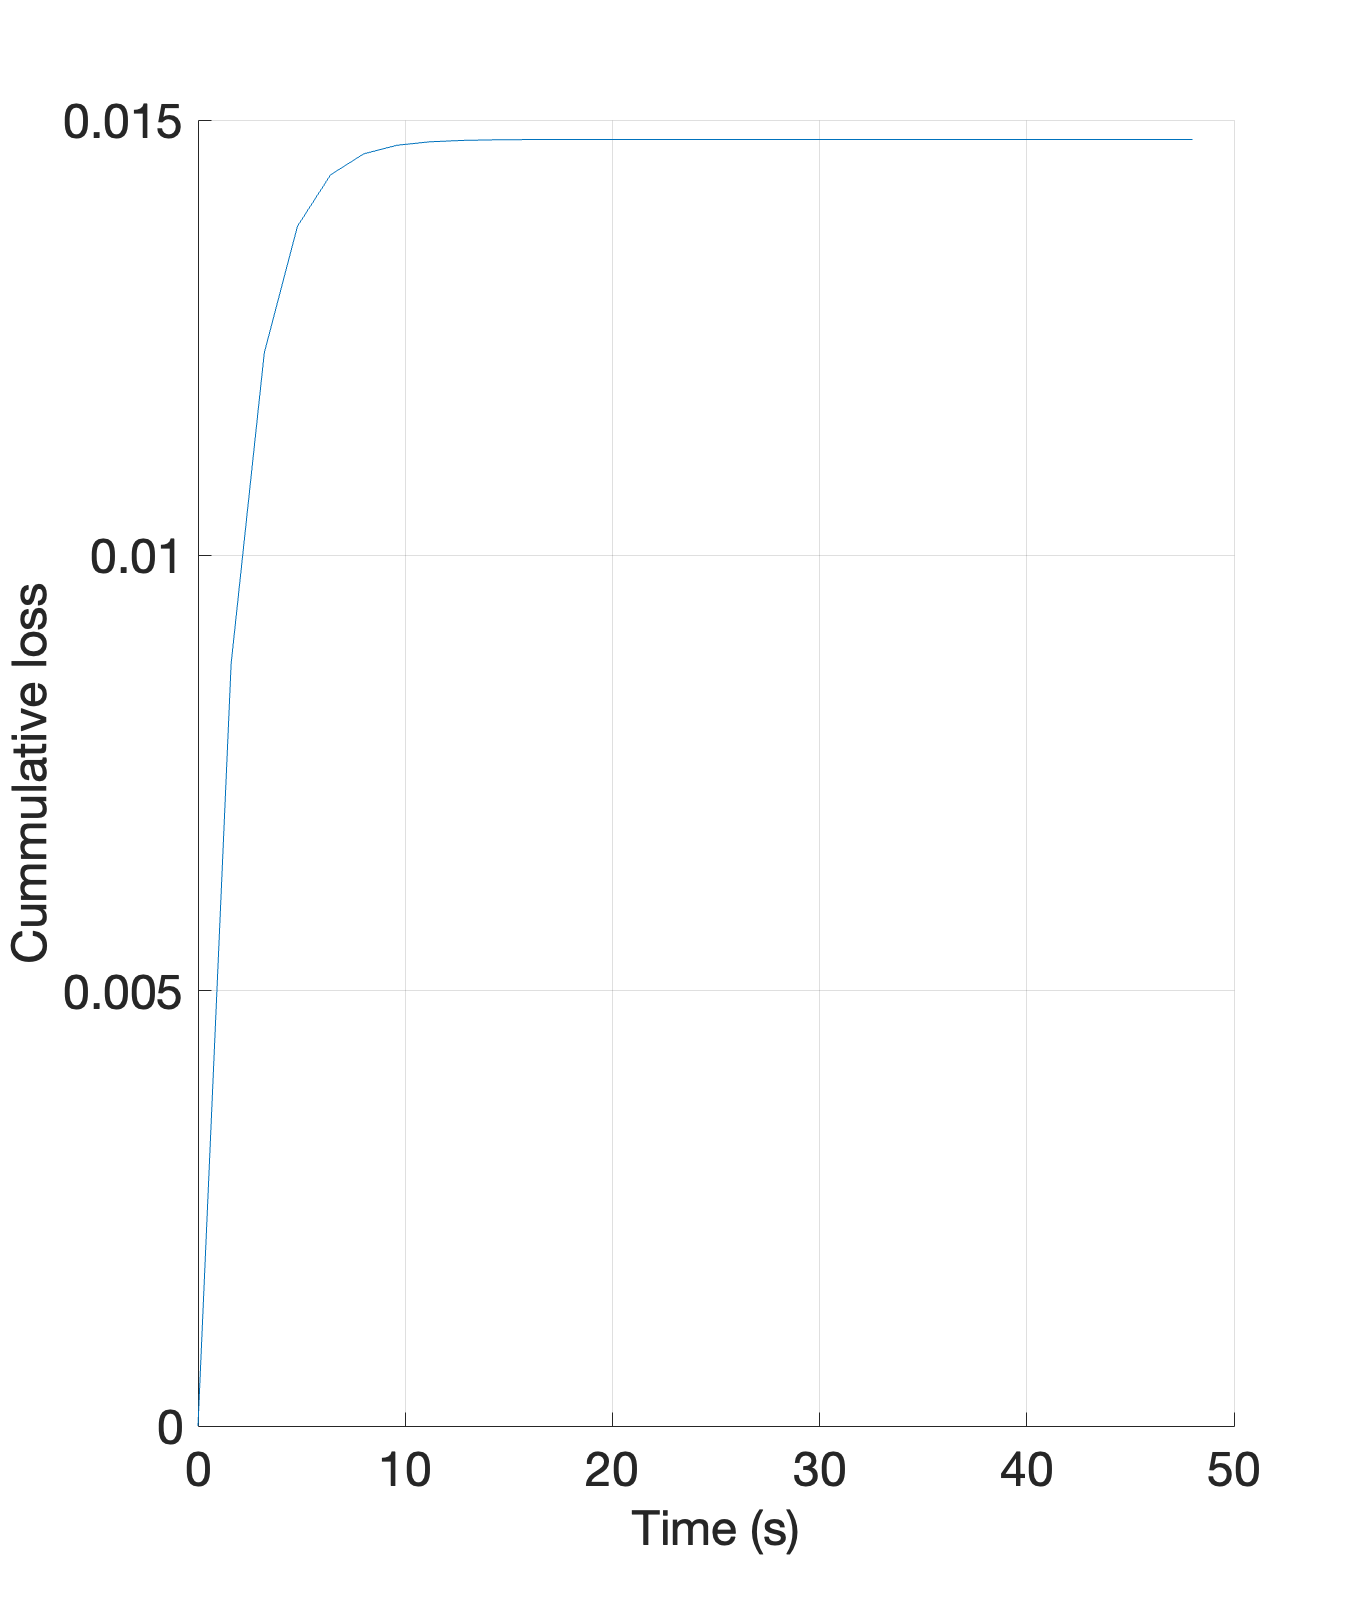
\includegraphics[width=\textwidth]{images/sstr12.png}
	\caption{Cummulative loss of Minimum variance controller}
	\label{fig:sstr12}
\end{figure}

\noindent The code for this section is available at \lstinline|assignment3/SSTR/SSTR_1.m|. 
